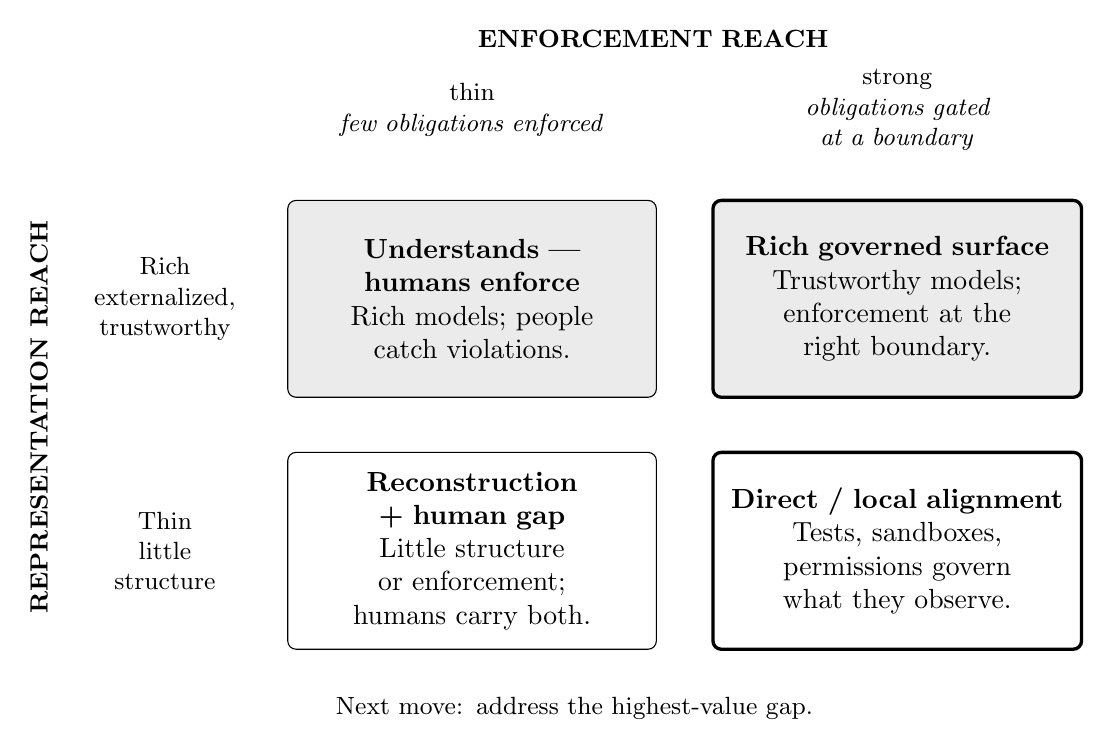
\begin{tikzpicture}[x=1cm,y=1cm,font=\magefigurefont\fontsize{10}{12}\selectfont,
box/.style={draw=black,fill=white,rounded corners=3pt,align=center,text width=3cm,minimum height=8mm,inner sep=4pt},
gate/.style={box,line width=1pt},note/.style={align=center,fill=white,inner sep=1pt,font=\magefigurefont\fontsize{9}{11}\selectfont},
edge/.style={-{Stealth[length=2mm]},line width=.6pt},optional/.style={edge,dashed},
every node/.style={text=black,execute at begin node={\hyphenpenalty=10000\exhyphenpenalty=10000}}]
\node[note,text width=10cm] (t5) at (1,1.8) {\textbf{ENFORCEMENT REACH}};
\node[note,text width=4cm] (t6) at (-1.3,0.9) {thin\\ \textit{few obligations enforced}};
\node[note,text width=4cm] (t7) at (4.1,0.9) {strong\\ \textit{obligations gated at a boundary}};
\node[note,rotate=90] at (-6.8,-3) {\textbf{REPRESENTATION REACH}};
\node[note,text width=2cm] (t9) at (-5.2,-1.5) {Rich\\ externalized,\\ trustworthy};
\node[note,text width=2cm] (t10) at (-5.2,-4.7) {Thin\\ little structure};
\node[box,minimum height=25mm,text width=4.4cm,fill=black!8] (a) at (-1.3,-1.5) {\textbf{Understands — humans enforce}\\ Rich models; people catch violations.};
\node[box,minimum height=25mm,text width=4.4cm,line width=1.2pt,fill=black!8] (b) at (4.1,-1.5) {\textbf{Rich governed surface}\\ Trustworthy models; enforcement at the right boundary.};
\node[box,minimum height=25mm,text width=4.4cm] (c) at (-1.3,-4.7) {\textbf{Reconstruction + human gap}\\ Little structure or enforcement; humans carry both.};
\node[box,minimum height=25mm,text width=4.4cm,line width=1.2pt] (d) at (4.1,-4.7) {\textbf{Direct / local alignment}\\ Tests, sandboxes, permissions govern what they observe.};
\node[note,text width=10cm] (t15) at (0,-6.7) {Next move: address the highest-value gap.};
\end{tikzpicture}
